% !TeX program = lualatex
\documentclass[12pt,oneside]{book}

% =======================
% Preambulo y metadatos
% =======================
% -------------------------------------------------------
% Paquetes Matemáticos
% -------------------------------------------------------
\usepackage{amsmath}
\usepackage{amssymb}
\usepackage{amsfonts}

% -------------------------------------------------------
% Paquetes de Algoritmos
% (Usar sólo algorithm2e que proporciona algoritmos y pseudocódigo)
% -------------------------------------------------------
% \usepackage{algorithm}      % Comentado: conflicto con algorithm2e
% \usepackage{algorithmic}    % Comentado: conflicto con algorithm2e

% Estilo adicional de pseudocódigo (ruled, vlined)
\usepackage[ruled,vlined]{algorithm2e}

% -------------------------------------------------------
% Control de figuras y posicionamiento
% -------------------------------------------------------
\usepackage{float}          % Permite la opción [H]
\usepackage{graphicx}

% -------------------------------------------------------
% TikZ para diagramas (requerido para 5.1.3)
% -------------------------------------------------------
\usepackage{tikz}
\usetikzlibrary{arrows.meta}
\usetikzlibrary{positioning}
\usetikzlibrary{shapes.geometric}
\usetikzlibrary{calc}

% -------------------------------------------------------
% Estética y microtipografía
% -------------------------------------------------------
\usepackage[protrusion=true,expansion=true]{microtype}
\usepackage{ragged2e}       % Mejor control de justificación
\raggedbottom               % Evita estiramientos verticales feos

% -------------------------------------------------------
% Ajuste de entornos tipo lista (para justificar texto)
% -------------------------------------------------------
\usepackage{etoolbox}
\AtBeginEnvironment{itemize}{\justifying}
\AtBeginEnvironment{enumerate}{\justifying}
\AtBeginEnvironment{description}{\justifying}

% -------------------------------------------------------
% Bibliografía (BibLaTeX + Biber)
% -------------------------------------------------------
\usepackage[
  backend=biber,
  style=numeric,
  sorting=none
]{biblatex}
\addbibresource{referencias.bib}

\input{metadata}

\begin{document}

% --------- Portada y preliminares ---------
\frontmatter
\begin{titlepage}
    \thispagestyle{empty}
    \begin{center}

        \vspace*{-1.5cm}

        % Título
        {\LARGE\bfseries
        Automatización en la Asignación de Tareas en un ERP para Talleres Industriales utilizando Algoritmos Genéticos\par}

        \vspace{0.8cm}

        % Logo abajo
        
\includegraphics[width=0.25\textwidth]{images/logopuj.png}\\[0.8cm]

        % Autores (sin códigos)
        {\large
        Maria José Pava Echeverry\\[0.15cm]
        Jose Daniel Ramirez Delgado\\}

        \vspace{0.8cm}

        % Directores
        {\large
        Directora:\\
        PhD. Gloria Ines Alvares Vargas\\[0.2cm]
        Co-director:\\
        PhD. Diego Luis Linares Ospina
        }
        
        \vfill

        % Facultad, programa, universidad y año (sin mes)
        {\large
        FACULTAD DE INGENIERÍA Y CIENCIAS\\
        INGENIERÍA DE SISTEMAS Y COMPUTACIÓN\\[0.3cm]
        \textbf{Pontificia Universidad Javeriana Cali}\\[0.2cm]
        Santiago de Cali, 2025
        }

    \end{center}
\end{titlepage}

\cleardoublepage
\input{frontmatter/resumen}
\cleardoublepage
\chapter*{Abstract}

This project develops and validates a genetic algorithm (GA) based model for automating task assignment in industrial workshop ERP systems. Manual task allocation in automotive technology workshops often results in worker overload, idle times, and delivery delays. The proposed GA-based approach integrates into the ERP work order management module, considering worker capabilities, spare parts availability, and workload distribution constraints.

The core problem is modeled as a variant of Job Shop Scheduling with practical constraints including task precedences, skill requirements, parts availability, and daily time horizons. The GA employs a dual-representation chromosome encoding both operator assignments and task sequencing priorities, evaluated through a fitness function that respects domain-specific constraints. The implementation uses Python 3.14.0, NumPy 1.26.4, and PyGAD 3.2.0, with calibrated parameters: 300 generations, population of 100, 15\% mutation rate, and ranking-based selection.

Experimental validation across 30 test instances from Rectificadora Recti-Ram workshop demonstrates significant advantages over the Shortest Processing Time (SPT) heuristic. The GA achieved 15.6\% reduction in makespan (157.37 vs 186.53 time units) and 14.3\% improvement in load balance (standard deviation 30.10 vs 35.11), while maintaining equivalent task completion rates. Both methods executed ~29.53 tasks daily, confirming quality gains stem from superior sequencing rather than increased capacity. The GA requires ~3.13 seconds per instance compared to milliseconds for SPT, yielding operationally viable computational costs.

Industrially, the 15.6\% efficiency gain represents approximately 29.16 additional productive minutes per day, equivalent to 117.6 annual hours. Improved load balance reduces bottlenecks, worker fatigue, and operational errors while enabling greater order volume capacity. This research contributes formalized methodology and reproducible solution using open-source tools, reducing adoption barriers for small and medium enterprises. Future extensions include hybrid metaheuristics, flexible job shop scheduling, multi-objective optimization, and Industry 4.0 integration.

Genetic algorithms demonstrate viability as practical tools for industrial task automation, outperforming classical heuristics while maintaining adaptability and reproducibility in real operational environments.



\cleardoublepage
\input{frontmatter/agradecimientos}
\cleardoublepage
\tableofcontents
\listoffigures
\listoftables

% --------- Cuerpo ---------
\mainmatter
\chapter{Introducción}

El presente proyecto de grado se centró en abordar los desafíos que enfrentan los talleres industriales en la gestión eficiente de sus operaciones, específicamente en la asignación de tareas dentro de un sistema de Planificación de Recursos Empresariales (ERP). La asignación tradicional de tareas, frecuentemente realizada de forma manual, puede conducir a ineficiencias significativas, tales como la sobrecarga de operarios, tiempos muertos en la producción y retrasos en las entregas, afectando directamente la productividad y la rentabilidad del taller.

En este contexto, la automatización de la asignación de tareas emerge como una solución crucial para optimizar el uso de los recursos y mejorar el flujo de trabajo. Este proyecto propuso el desarrollo de un modelo de automatización basado en algoritmos genéticos, una técnica de inteligencia artificial que ha demostrado su eficacia en la resolución de problemas complejos de optimización. Al implementar algoritmos genéticos en el módulo de gestión de órdenes de trabajo de un ERP, se buscó automatizar la distribución de tareas considerando variables clave como las capacidades técnicas de los operarios, la disponibilidad de insumos y la carga de trabajo actual.

Para el desarrollo del proyecto, se llevó a cabo un proceso metodológico que incluyó el análisis de los procesos actuales de asignación de tareas en Rectificadora Recti-Ram, la recopilación y estructuración de datos operacionales, el diseño e implementación de un algoritmo genético adaptado a las necesidades específicas del taller, y la evaluación comparativa del modelo propuesto frente a la heurística clásica \textit{Shortest Processing Time} (SPT), ampliamente utilizada en el campo de la ingeniería industrial. Los resultados obtenidos demostraron que el algoritmo genético desarrollado logró una reducción del 15.6\% en el makespan promedio (de 186.53 a 157.37 unidades de tiempo) y una disminución del 14.3\% en la desviación estándar de carga entre operarios (de 35.11 a 30.10), logrando cronogramas más compactos, mejor balance de trabajo y mayor estabilidad operativa. Estas mejoras validaron la eficacia y aplicabilidad del enfoque propuesto en un entorno industrial real, demostrando que el algoritmo genético no solo es competitivo frente a métodos tradicionales, sino que los supera en los aspectos más relevantes para la operación diaria del taller.

La investigación se llevó a cabo en colaboración con la empresa Rectificadora Recti-Ram, lo que proporcionó un contexto real y datos relevantes para el desarrollo y la validación del modelo.

A través de este proyecto, se contribuyó al avance en la automatización de los talleres industriales, proporcionando una herramienta que permite mejorar la eficiencia operativa, reducir los costos y aumentar la satisfacción del cliente mediante la optimización de los procesos de asignación de tareas.
\chapter{Definición y Planteamiento del Problema}

\section{Planteamiento del Problema}

El entorno productivo de los talleres industriales enfrenta diversas problemáticas que afectan su eficiencia y rendimiento. Entre los principales desafíos se encuentran la capacidad de producción limitada, los largos tiempos de fabricación y los retrasos en las fechas de entrega \cite{ref7}. Además, la falta de sistemas estructurados para la evaluación de calidad y la baja integración tecnológica pueden impactar negativamente la productividad del proceso \cite{ref7}.  

La asignación de tareas en los talleres industriales es un factor clave para optimizar el uso de recursos humanos y técnicos. Una planificación ineficiente puede provocar retrasos, una distribución desequilibrada de la carga de trabajo y una reducción en la productividad \cite{ref8}. La complejidad de estos entornos productivos, caracterizados por la variabilidad en la demanda y la necesidad de coordinar múltiples operaciones, hace necesario el uso de enfoques avanzados que permitan gestionar eficazmente la distribución de actividades y mejorar el cumplimiento de los plazos de entrega \cite{ref8}.  

Para abordar este problema, se propone la implementación de algoritmos genéticos (AG) en un módulo ERP de gestión de órdenes de trabajo. Esta solución permitirá automatizar la distribución de tareas considerando factores clave como:

\begin{itemize}
    \item Capacidades técnicas de cada operario.
    \item Disponibilidad de insumos requeridos para cada tarea.
    \item Carga de trabajo actual y disponibilidad horaria de los operarios.
\end{itemize}

Adicionalmente, este estudio evaluará el desempeño del algoritmo genético en comparación con otro método de optimización utilizado en ingeniería industrial, con el objetivo de determinar su viabilidad y eficacia en este contexto.


\subsection{Formulación}
¿Cómo mejorar la asignación de tareas en un ERP de talleres industriales utilizando algoritmos genéticos, y cómo se compara su rendimiento con otras técnicas de automatización utilizadas en ingeniería industrial?

\subsection{Sistematización}
Para abordar de manera integral el problema de investigación, se plantean las siguientes preguntas:

\begin{enumerate}
    \item ¿Cuáles son los principales factores que afectan la asignación de tareas en talleres industriales?
    \item ¿Cómo pueden los algoritmos genéticos mejorar la automatización de tareas dentro del ERP?
    \item ¿Qué otras técnicas de automatización existen en ingeniería industrial para resolver problemas similares?
    \item ¿Cómo se comparan los resultados obtenidos con algoritmos genéticos respecto a otra técnica de automatización en términos de eficiencia y calidad de la solución?
\end{enumerate}

\section{Objetivos}

\subsection{Objetivo General} 
Desarrollar un modelo de automatización basado en algoritmos genéticos para apoyar en el módulo de asignación de tareas de un sistema ERP de talleres industriales, comparándolo con otro método de automatización utilizado en ingeniería industrial.

\subsection{Objetivos Específicos}
Para alcanzar el objetivo general, se plantean los siguientes objetivos específicos:

\begin{enumerate}
    \item Identificar las caracaterísticas claves que influyen en la asignación de tareas en talleres industriales.
    \item Diseñar e implementar un modelo utilizando un algoritmo genético para automatizar la asignación de tareas tales como desmontaje del motor, limpieza y diagnóstico, rectificación de cilindros, rectificación de cigüeñales, ajuste de válvulas, ensamblaje y prueba del motor.
    \item Evaluar la funcionalidad del modelo y el desempeño del algoritmo genético en comparación con otra técnicas de automatización utilizadas en ingeniería industrial.
    \item Analizar los beneficios y limitaciones de los algoritmos genéticos en este contexto.
\end{enumerate}

\section{Justificación}

La gestión eficiente de órdenes de trabajo en talleres industriales impacta directamente la productividad y rentabilidad. El uso de algoritmos genéticos puede ofrecer una solución flexible y adaptable que automatiza los tiempos de ejecución, minimiza costos y mejora la distribución equitativa de la carga de trabajo.  

La empresa Rectificadora Recti-Ram  cuenta con datos históricos sobre tiempos de reparación, asignación de operarios y disponibilidad de recursos, lo que facilita el entrenamiento y validación del modelo propuesto. Asimismo, la disponibilidad de la empresa para proporcionar información clave sobre su flujo de trabajo y sus restricciones operativas permitirá diseñar un modelo que se ajuste a las necesidades reales.  

Además, comparar esta solución con otro método de automatización permitirá validar su aplicabilidad en escenarios industriales reales, asegurando que la mejor estrategia sea implementada dentro del ERP del taller, garantizando así una planificación eficiente y adaptable a las condiciones dinámicas del entorno productivo.

\section{Delimitaciones y Alcances}

\begin{itemize}
    \item Se enfocará en la asignación de tareas dentro del módulo de ordenes de trabajo en un ERP para talleres industriales.
    \item Se implementará un modelo basado en algoritmos genéticos.
    \item Se comparará con otro método de automatización (a definir en consulta con expertos en ingeniería industrial).
\end{itemize}
\chapter{Marco de Referencia}

\section{Marco Teórico}
Para comprender el desarrollo de un módulo de ERP destinado a la automatización de la asignación de tareas en un taller industrial, es esencial establecer una base teórica sólida sobre los conceptos clave involucrados. Este proyecto se enfoca en la aplicación de algoritmos genéticos como una técnica de inteligencia artificial que permite la automatización de procesos de toma de decisiones en entornos industriales. Los algoritmos genéticos permiten analizar múltiples combinaciones posibles para la asignación de recursos y actividades, facilitando la gestión eficiente de órdenes de trabajo en un ERP.

Dentro del campo de la ingeniería industrial, se han desarrollado diversas metodologías para mejorar la productividad y la gestión de recursos, muchas de ellas basadas en principios de automatización y sistemas inteligentes. En este proyecto, se desarrollará un módulo de ERP que empleará algoritmos genéticos para la automatización de la asignación de tareas, permitiendo reducir la intervención manual y mejorar la eficiencia operativa en talleres industriales. A lo largo del estudio, se comparará este enfoque con otras metodologías existentes en la industria, evaluando su desempeño en términos de tiempos de procesamiento, flexibilidad y adaptabilidad a escenarios reales.

Los sistemas ERP (Enterprise Resource Planning) son herramientas integradas que permiten la automatización y gestión de los procesos empresariales esenciales, tales como finanzas, producción, logística y ventas. Un ERP centraliza la información empresarial, optimizando la toma de decisiones y reduciendo la fragmentación de datos, lo que mejora la eficiencia operativa. Estos sistemas han evolucionado desde los sistemas MRP (Material Requirements Planning) y actualmente constituyen una pieza clave en la digitalización de la industria \cite{ref1}.

\subsection{Automatización con ERP en talleres industriales}

La implementación de ERP en talleres industriales responde a la necesidad de automatizar y estructurar procesos que, de otro modo, se gestionarían de forma manual, lo que puede generar ineficiencias. En los talleres de tecnomecánica, donde se requiere un control riguroso de los repuestos y tiempos de trabajo, un ERP automatizado permite la asignación eficiente de tareas según la disponibilidad de operarios y recursos, reduciendo tiempos de espera y mejorando la productividad. 

En un estudio realizado en 2019 \cite{ref2}, se identificó que el 70.4\% de las quejas de los clientes en una compañía analizada estaban relacionadas con retrasos en la entrega de órdenes de trabajo, mientras que el 29.6\% restante correspondía a problemas de órdenes no confirmadas y reprocesos. Estos problemas, comunes en talleres industriales, pueden ser mitigados mediante un ERP que automatice la distribución de tareas y optimice la administración de recursos, minimizando errores humanos y mejorando la trazabilidad de las órdenes de trabajo.

\subsection{Algoritmos Genéticos (GA) para la Automatización}

La automatización de procesos en entornos industriales ha avanzado con el uso de algoritmos evolutivos, entre los cuales los algoritmos genéticos (GA) han demostrado ser eficaces para resolver problemas de asignación de tareas y planificación de recursos. Estos algoritmos, inspirados en la selección natural y la evolución biológica, trabajan con poblaciones de soluciones potenciales, aplicando operadores como la selección, el cruce (crossover) y la mutación para encontrar soluciones óptimas de manera iterativa \cite{ref3}.

A diferencia de los métodos tradicionales de asignación de tareas, que pueden depender de reglas predefinidas y cálculos deterministas, los algoritmos genéticos ofrecen una solución flexible que se adapta dinámicamente a cambios en el entorno de producción. Gracias a su capacidad de explorar múltiples combinaciones de asignación de tareas y su enfoque probabilístico, los GA pueden reducir tiempos improductivos y mejorar la distribución del trabajo en talleres industriales.

\section{Técnicas de Automatización en Ingeniería Industrial}

La automatización en la ingeniería industrial ha evolucionado con el desarrollo de metodologías como Lean Manufacturing, Six Sigma y la investigación de operaciones, las cuales buscan mejorar la eficiencia mediante la eliminación de desperdicios, la reducción de variabilidad en los procesos y la optimización de los flujos de trabajo \cite{ref4}. Estas estrategias han sido aplicadas con éxito en la manufactura y la gestión industrial, mejorando la toma de decisiones y la productividad.

En este proyecto, el enfoque se basa en la automatización de la asignación de tareas dentro de un ERP mediante inteligencia artificial, permitiendo gestionar dinámicamente la carga de trabajo de los operarios según la demanda y la disponibilidad de recursos. A diferencia de las metodologías tradicionales, que dependen de reglas fijas y modelos matemáticos estrictos, este enfoque permite una mayor flexibilidad y adaptación a entornos productivos cambiantes, mejorando la eficiencia operativa en los talleres industriales.

\section{Antecedentes}

La programación de tareas en entornos industriales ha sido un campo de estudio ampliamente abordado en la literatura debido a la complejidad inherente de problemas como Flow Shop, Job Shop y Flexible Job Shop, todos ellos catalogados como NP-hard \cite{flowshop,flexjobshop}. Esta complejidad ha motivado el desarrollo de metodologías basadas en heurísticas, reglas de despacho y metaheurísticas avanzadas para obtener soluciones eficientes dentro de límites computacionales razonables. En este contexto, los algoritmos genéticos (AG) han demostrado un rendimiento destacado en la optimización de tareas, especialmente en escenarios donde múltiples restricciones interactúan entre sí.

Uno de los trabajos más relevantes es el de Delgado et al. \cite{Delgado2005}, quienes propusieron un algoritmo genético para la programación de tareas en una celda de manufactura y compararon su desempeño con métodos heurísticos tradicionales. Sus resultados mostraron que los AG pueden reducir tiempos improductivos y mejorar la utilización de recursos, destacando su capacidad para explorar soluciones que las reglas de prioridad no alcanzan debido a su naturaleza determinista.

De manera complementaria, Meisel y Prado \cite{meisel2010} desarrollaron un algoritmo genético híbrido que incorpora enfriamiento simulado, demostrando que las metaheurísticas híbridas pueden ofrecer soluciones más estables y de mayor calidad en problemas de tipo Job Shop. Este estudio respalda la idea de que los AG son especialmente adecuados para problemas con múltiples restricciones, como precedencias, máquinas en paralelo y tiempos variables de procesamiento.

En el ámbito de la automatización industrial desde la perspectiva de Industria 4.0, Zhang et al. \cite{industry4} presentan un análisis del estado del arte de algoritmos evolutivos aplicados a la programación en sistemas inteligentes. Su investigación concluye que los AG, junto con técnicas híbridas de optimización, son herramientas clave para la toma de decisiones en entornos altamente dinámicos y automatizados. Esta tendencia refuerza la pertinencia del uso de AG como enfoque moderno para la gestión de recursos en talleres industriales.

En cuanto a la asignación de tareas en problemas de tipo Task Assignment Problem (TAP), Savić et al. \cite{ref10} demostraron que los AG pueden encontrar soluciones óptimas o cercanas al óptimo en espacios de búsqueda complejos, superando métodos deterministas y heurísticos en términos de tiempo de ejecución y calidad de resultados. De forma similar, Wang \cite{ref9} aplicó algoritmos genéticos al diseño automático de maquinaria, mostrando mejoras significativas frente a métodos tradicionales en precisión y tiempos de procesamiento.

Por otra parte, investigaciones sobre heurísticas industriales, como las reglas de despacho SPT, EDD y FCFS, han demostrado ser métodos simples y eficientes para problemas básicos de secuenciación, pero con limitaciones marcadas en problemas con múltiples restricciones o estructuras complejas de precedencia \cite{valletesis,flowshop}. Esta brecha entre simplicidad y capacidad de adaptación es precisamente lo que motiva la comparación entre SPT y algoritmos evolutivos en el presente estudio.

En conjunto, estos antecedentes evidencian que los algoritmos genéticos han sido utilizados con éxito en diversos dominios de la optimización industrial, mientras que las heurísticas tradicionales siguen siendo herramientas fundamentales como métodos comparativos o de referencia. En el caso particular de un taller industrial basado en un sistema ERP, la literatura existente es limitada. Por ello, el presente proyecto aporta un enfoque novedoso al integrar un algoritmo genético dentro de un entorno simulado que replica el flujo real de un taller automotriz, comparándolo directamente con una heurística industrialmente aceptada como SPT. Esta comparación permite evaluar el potencial de los AG para mejorar la asignación de tareas y la eficiencia operativa en un contexto aplicado.


\chapter{Formalización del problema}

El presente capítulo describe la estructura formal del problema de programación diaria del taller industrial,
incluyendo la caracterización del flujo operativo, la definición matemática de los elementos que componen el
sistema y la modelación del comportamiento del taller bajo sus restricciones reales. Los elementos
descriptivos del funcionamiento real del taller se documentan en el capítulo de Marco de Referencia;
aquí se retoman como insumo para la formulación matemática. Esta formalización constituye la base para
el desarrollo posterior del algoritmo genético y el método SPT, presentados en los capítulos siguientes.

\section{Estudio del flujo de trabajo del taller industrial}

El taller de reparación de motores opera bajo un flujo secuencial condicionado por restricciones de precedencia,
disponibilidad de repuestos, habilidades del personal e interacción entre tareas dentro de una misma orden
de trabajo. Cada día se recibe un conjunto de órdenes de trabajo que agrupan tareas mecánicas con distintos
requerimientos técnicos, y el objetivo operativo es completar la mayor cantidad posible de dichas tareas dentro
de la jornada laboral.

Operativamente, la jornada sigue el siguiente comportamiento conceptual:
\begin{enumerate}
    \item Llegan varias órdenes de trabajo, cada una con un conjunto de operaciones asociadas.
    \item Se identifican los recursos requeridos para cada operación: operarios aptos y repuestos específicos.
    \item Algunas tareas deben esperar a que otras concluyan dentro de una misma orden.
    \item Los operarios ejecutan las tareas secuencialmente dentro del horizonte diario disponible.
    \item Se prioriza maximizar el número de tareas completadas sin violar las restricciones operativas.
\end{enumerate}

Este flujo describe el contexto real que posteriormente se formaliza para alimentar la simulación y los algoritmos
 de optimización.

\subsection{Ejemplo de Estructura de Precedencias en una Orden Real}

La Figura~\ref{fig:precedencias-orden-real} muestra la estructura de dependencias de una orden de trabajo real del taller. Cada nodo representa una tarea con su identificador y nombre, mientras que las flechas direccionadas indican la relación de precedencia: una tarea solo puede iniciarse una vez que sus tareas predecesoras hayan sido completadas. Este tipo de restricciones son típicas en procesos de reparación de motores, donde ciertas operaciones (como pruebas de funcionamiento) deben realizarse al final, y otras (como rimar guías) pueden ejecutarse en paralelo siempre que no sea por el mismo operario. El diagrama ilustra cómo las restricciones de precedencia generan un grafo dirigido acíclico (DAG) que debe ser respetado durante la programación de las tareas.

\begin{figure}[H]
\centering
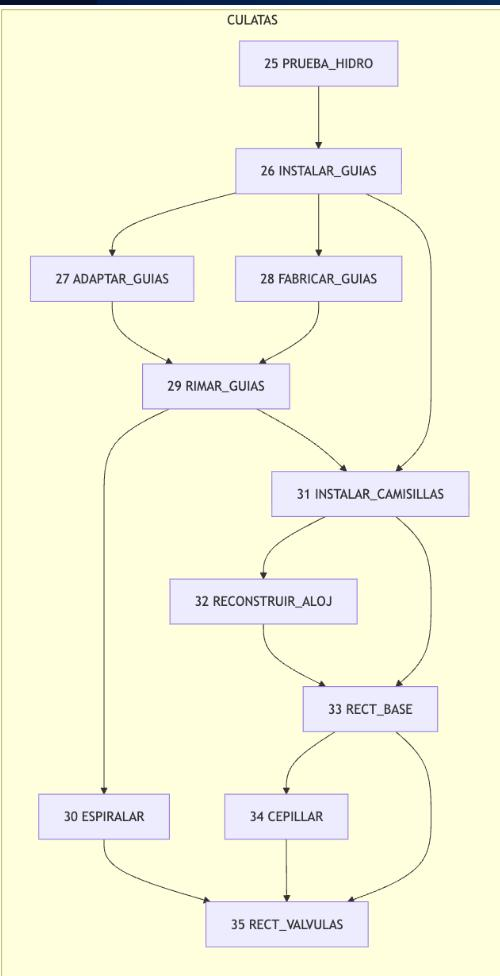
\includegraphics[width=0.65\textwidth]{figures/diagrama_tareas.jpg}
\caption{Estructura de precedencias de una orden de trabajo real del taller. Los nodos representan tareas identificadas por número y nombre, y las flechas indican relaciones de dependencia donde una tarea no puede iniciarse hasta que todas sus predecesoras hayan sido completadas. Este grafo dirigido acíclico es típico en procesos de reparación de motores.}
\label{fig:precedencias-orden-real}
\end{figure}

\section{Supuestos operativos y alcance}

Los supuestos del modelo parten de la caracterización levantada con el taller Recti-Ram. Se considera que:
\begin{itemize}
    \item La duración base de cada tipo de tarea es conocida y corresponde a tiempos promedio validados con expertos.
    \item Las habilidades de cada operario son estáticas durante la jornada y definen qué tareas puede ejecutar.
    \item Las precedencias sólo aplican dentro de una misma orden de trabajo.
    \item La disponibilidad de repuestos se conoce al inicio del día y se representa mediante parámetros binarios.
    \item Cada operario cuenta con un horizonte máximo de 480 minutos, equivalente a una jornada de 8 horas.
\end{itemize}

Estos supuestos delimitan el alcance del problema y sirven como base para la formalización matemática descrita a
continuación.

\section{Formalización Matemática del Problema}

\subsection{Conjuntos y parámetros fundamentales}

La estructura formal se define sobre los conjuntos:
\[
\begin{aligned}
OT &= \{1, \dots, m\} && \text{Órdenes de trabajo},\\
T_d &= \{1, \dots, n\} && \text{Tareas concretas del día},\\
O &= \{1, \dots, r\} && \text{Operarios disponibles},\\
T &= \{1, \dots, q\} && \text{Tipos de tarea identificados}.
\end{aligned}
\]

Los parámetros que caracterizan el sistema son:
\[
\begin{aligned}
p(t) &: T \rightarrow \mathbb{N} && \text{Duración base del tipo } t,\\
E(t) &\subseteq O && \text{Operarios aptos para el tipo } t,\\
P(t) &\subseteq T && \text{Tipos que deben preceder a } t,\\
R_{ot} &\in \{0,1\}^{|T|} && \text{Disponibilidad de repuestos por orden},\\
H &= 480 && \text{Horizonte diario en minutos}.
\end{aligned}
\]

Para cada tarea \(i \in T_d\) se conocen los parámetros \(ot(i) \in OT\) y \(tipo(i) \in T\).

\subsection{Variables de decisión y auxiliares}

La formalización utiliza el siguiente conjunto de variables:
\begin{itemize}
    \item \(x_i \in \{0,1\}\): indica si la tarea \(i\) se ejecuta dentro del horizonte.
    \item \(a_i \in O\): operario asignado a la tarea \(i\).
    \item \(s_i \geq 0\) y \(f_i = s_i + p(tipo(i))\): inicio y fin de la tarea \(i\).
    \item \(tpo_o \geq 0\): tiempo acumulado utilizado por el operario \(o\).
    \item \(comp_{ot}\): conjunto de tipos ya completados en la orden \(ot\).
    \item \(occ_{ot}\): conjunto de intervalos ocupados por tareas aceptadas dentro de la orden \(ot\).
\end{itemize}

Las tres últimas variables operan como estados auxiliares dentro de la simulación y permiten verificar factibilidad
al evaluar cada cronograma candidato.

\subsection{Estructura temporal}

El tiempo se modela como un intervalo continuo \([0, H]\). Cada tarea \(i\) programada por el operario \(a_i\) ocupa el
intervalo \([s_i, f_i)\), donde \(f_i = s_i + p(tipo(i))\). El tiempo acumulado por operario se actualiza mediante
\(tpo_{a_i} \gets f_i\) cuando se acepta la tarea, garantizando que la jornada individual no exceda \(H\).

\subsection{Restricciones operativas formales}

La factibilidad de una solución requiere cumplir simultáneamente las siguientes restricciones:
\begin{align}
a_i &\in E(tipo(i)) && \forall i \in T_d \label{cons:aptitud} \\
R_{ot(i)}(tipo(i)) &\geq x_i && \forall i \in T_d \label{cons:repuestos} \\
P(tipo(i)) &\subseteq comp_{ot(i)} && \forall i \in T_d \text{ con } x_i = 1 \label{cons:precedencia} \\
f_i &\leq H && \forall i \in T_d \label{cons:horizonte} \\
[s_i, f_i) &\cap occ_{ot(i)} = \emptyset && \forall i \in T_d \text{ con } x_i = 1 \label{cons:solape}
\end{align}

La restricción \eqref{cons:aptitud} garantiza que cada tarea se asigne a un operario competente, mientras que
\eqref{cons:repuestos} asegura la existencia de repuestos antes de iniciar la operación. La relación de precedencia
\eqref{cons:precedencia} obliga a que los tipos requeridos se encuentren en el conjunto de tareas completadas de la
misma orden. La cota temporal \eqref{cons:horizonte} impide exceder la jornada y \eqref{cons:solape} evita traslapos entre
tareas pertenecientes a la misma orden de trabajo.

Adicionalmente, la coherencia entre la variable binaria \(x_i\) y el cronograma se mantiene mediante las implicaciones:
\[
\begin{aligned}
x_i = 0 &\Rightarrow a_i \text{ y } s_i \text{ quedan sin asignar},\\
x_i = 1 &\Rightarrow s_i = tpo_{a_i}, \quad f_i = s_i + p(tipo(i)).
\end{aligned}
\]

\subsection{Definición formal del problema de optimización}

El objetivo operativo consiste en maximizar el número de tareas completadas durante la jornada, lo cual se expresa como:
\[
\begin{aligned}
\max_{x,a,s} \quad & \sum_{i \in T_d} x_i \\
\text{s.a.} \quad & \text{Restricciones \eqref{cons:aptitud}--\eqref{cons:solape}}, \\
& x_i \in \{0,1\}, \; a_i \in O, \; s_i \geq 0, \quad \forall i \in T_d.
\end{aligned}
\]

La solución del problema proporciona un cronograma factible que respeta las reglas industriales y utiliza de forma
 eficiente la capacidad diaria disponible.

\section{Representación computacional del sistema}

Para ejecutar la simulación y alimentar los algoritmos, la formalización anterior se implementa mediante una
configuración digital que integra todos los elementos estructurales del taller:
\begin{itemize}
    \item \textbf{Catálogo de tareas}: lista de los tipos contenidos en \(T\), cada uno con su duración base \(p(t)\) y la
    familia operativa correspondiente.
    \item \textbf{Matriz de habilidades}: representación explícita de \(E(t)\), indicando qué operarios están calificados para
    cada tipo de tarea.
    \item \textbf{Relaciones de precedencia}: estructuras de datos que codifican \(P(t)\) y permiten validar dependencias dentro
    de una misma orden.
    \item \textbf{Parámetros diarios}: conjunto de tareas \(T_d\), asociación con órdenes \(ot(i)\) y disponibilidad de repuestos
    \(R_{ot}\) derivada del levantamiento de información real.
    \item \textbf{Horizonte y estados auxiliares}: valores iniciales de \(tpo_o\), \(comp_{ot}\) y \(occ_{ot}\) que se actualizan
    durante la evaluación de cada solución.
\end{itemize}

Esta representación computacional garantiza consistencia entre la formalización matemática y el comportamiento del
simulador que se utiliza en los capítulos posteriores para evaluar SPT y el algoritmo genético.

\chapter{Desarrollo de la Solución}

\section{Aqui comenzamos }

El problema se formula como un problema de asignación y secuenciación de tareas sujeto a múltiples restricciones operativas. El objetivo general consiste en maximizar el número de tareas programadas dentro de un horizonte diario de 8 horas por operario, garantizando la factibilidad respecto a precedencias, disponibilidad de repuestos y cualificación del personal.

\subsection{Variables}

\textbf{Variables de decisión:}

\begin{itemize}
    \item $y_i$: operario asignado a la tarea $i$, donde $y_i \in E(\mathrm{tipo}(i))$.
    \item $\pi_i \in [0,1]$: prioridad asignada a la tarea $i$ para determinar su orden de intento de programación.
\end{itemize}

\textbf{Variables auxiliares utilizadas en la simulación:}

\begin{itemize}
    \item $tpo[o]$: tiempo total utilizado por el operario $o$.
    \item $\mathrm{comp}[ot]$: conjunto de tareas completadas dentro de la orden de trabajo $ot$.
    \item $\mathrm{occ}[ot]$: intervalos ocupados en la orden de trabajo $ot$.
\end{itemize}

\subsection{Restricciones}

\begin{itemize}
    \item \textbf{Aptitud del operario:}  
    $y_i \in E(\mathrm{tipo}(i))$.
    \item \textbf{Disponibilidad de repuesto:}  
    Solo puede programarse una tarea si el repuesto asociado a su orden de trabajo está disponible.
    \item \textbf{Precedencias internas de la misma OT:}  
    \[
        \forall t' \in (\mathcal{P}(\mathrm{tipo}(i)) \cap \text{OT}(i)): \; t' \in \mathrm{comp}[\mathrm{ot}(i)]
    \]
    \item \textbf{Horizon­te máximo diario:}  
    $f_i \leq H$.
    \item \textbf{No solapamiento dentro de la misma OT:}  
    \[
        \neg (s_i < f' \land f_i > s'), \quad \forall [s', f') \in \mathrm{occ}[\mathrm{ot}(i)]
    \]
\end{itemize}

\subsection{Función Objetivo}

La función objetivo maximiza el número de tareas programadas y penaliza violaciones a las restricciones:

\[
\operatorname{fitness} =
100 N_{\text{exec}}
- 10 P_{\text{prec}}
- 10 P_{\text{rep}}
- 15 P_{\text{apt}}
- 12 P_{\text{ot}}
- 0.1 E_{\text{hor}}
- 0.5 \sigma
- 0.1 C_{\max}
\]

donde los términos representan:  
$N_{\text{exec}}$ tareas ejecutadas,  
$P_{\text{prec}}$ violaciones de precedencia,  
$P_{\text{rep}}$ faltas de repuestos,  
$P_{\text{apt}}$ asignaciones a operarios no aptos,  
$P_{\text{ot}}$ solapamientos en la misma orden,  
$E_{\text{hor}}$ excede del horizonte,  
$\sigma$ desviación estándar (balance de carga),  
$C_{\max}$ makespan.

% --------------------------------------------------------

\section{Diseño del Algoritmo Genético}

El algoritmo genético se diseñó para explorar combinaciones de asignación y secuenciación que respeten la estructura operativa del taller. Cada individuo representa un cronograma potencial que es evaluado mediante una simulación determinista.

\subsection{Representación}

Cada individuo se define como un vector de $2n$ dimensiones:

\[
[\, y_1, \dots, y_n \,] \;\Vert\; [\, \pi_1, \dots, \pi_n \,]
\]

\begin{itemize}
    \item Primeros $n$ genes: operario asignado, restringido al conjunto $E(\mathrm{tipo}(i))$.
    \item Últimos $n$ genes: prioridades en $[0,1]$.
\end{itemize}

\subsection{Selección}

Se empleó selección por \textbf{ranking}, adecuada para entornos donde la distribución de aptitud puede ser muy desigual debido a penalizaciones fuertes.

\subsection{Cruce}

Se utilizó cruce de tipo \textbf{single\_point}, apropiado debido a que el cromosoma posee dos mitades homogéneas: asignación y prioridad.

\subsection{Mutación}

Mutación aleatoria sobre el \textbf{15\%} de los genes:

\begin{itemize}
    \item Para asignaciones: se elige aleatoriamente un nuevo operario dentro de $E(\mathrm{tipo}(i))$.
    \item Para prioridades: se asigna un valor continuo uniforme en $[0,1]$.
\end{itemize}

\subsection{Parámetros}

\begin{itemize}
    \item Generaciones: 250
    \item Población: 100 individuos
    \item Padres por generación: 10
    \item Padres preservados: 5
    \item Semilla: 42 (reproducibilidad)
\end{itemize}

\subsection*{Evaluación del Individuo}

La simulación determina:

\begin{itemize}
    \item tareas ejecutadas,
    \item tareas rechazadas por precedencias, repuestos, aptitud o solapamiento,
    \item balance de carga entre operarios,
    \item makespan del sistema.
\end{itemize}

% --------------------------------------------------------

\section{Implementación del Método SPT}

Texto pendiente.

% --------------------------------------------------------

\section{Integración con el Entorno Simulado}

Texto pendiente.

% --------------------------------------------------------

\section{Arquitectura General del Sistema Desarrollado}

Texto pendiente.


\chapter{Resultados Experimentales}
\label{chap:ejecucion-obtencion-resultados}


\section{Configuración Final del AG}

A partir del proceso de calibración presentado en las subsecciones anteriores ---donde se evaluaron de forma independiente el operador de cruce, el número de generaciones y la probabilidad de mutación--- se obtuvo una configuración final del algoritmo genético que equilibra de manera adecuada la calidad de las soluciones y el costo computacional. Esta configuración fue utilizada en todas las comparaciones realizadas posteriormente contra el método SPT en el Capítulo~7.

En síntesis, la calibración determinó que:

\begin{itemize}
    \item El operador de cruce \textit{single\_point} ofrece el mejor desempeño en un horizonte amplio de 480 minutos, superando consistentemente a \textit{two\_points}.
    \item Un número de \textbf{300 generaciones} es suficiente para que el algoritmo converja hacia soluciones de alta calidad, mientras que valores mayores no aportan mejoras significativas y pueden incluso degradar el rendimiento.
    \item Una probabilidad de mutación del \textbf{15\%} logra el mejor equilibrio entre exploración y explotación del espacio de búsqueda, evitando tanto la convergencia prematura (como sucede con 5\%) como la pérdida de estabilidad evolutiva (observada con 25\%).
\end{itemize}

Con base en estos resultados, la configuración final del algoritmo genético utilizada en las simulaciones comparativas es la siguiente:

\begin{table}[htbp]
\centering
\small
\caption{Configuración final seleccionada para el algoritmo genético.}
\label{tab:config-final-ag}
\begin{tabular}{@{}lc@{}}
\toprule
\textbf{Parámetro} & \textbf{Valor seleccionado} \\
\midrule
Operador de cruce & \textit{single\_point} \\
Número de generaciones & 300 \\
Tamaño de población & 100 \\
Método de selección & \textit{rank} \\
Padres por generación & 10 \\
Padres preservados & 5 \\
Probabilidad de mutación & 15\% \\
Semilla aleatoria & 42 \\
\bottomrule
\end{tabular}
\end{table}

Esta configuración proporciona un desempeño robusto en términos de tareas ejecutadas, carga total y estabilidad del proceso evolutivo. Además, se mantiene dentro de límites razonables de tiempo de ejecución, lo que facilita su aplicación práctica en un taller industrial. Los experimentos del capítulo siguiente emplean exclusivamente esta configuración, garantizando que la comparación frente al método SPT se realice bajo condiciones justas y reproducibles.

\chapter{Análisis de Resultados}
\label{chap:analisis-resultados}

Este capítulo presenta el análisis de los resultados obtenidos en la comparación entre el Algoritmo Genético (AG) y la heurística clásica \textit{Shortest Processing Time} (SPT). El objetivo es evaluar el desempeño de ambos métodos bajo condiciones realistas del taller, utilizando métricas relevantes para la programación diaria de tareas y considerando indicadores exclusivamente operativos.

El análisis combina una perspectiva técnica—basada en métricas cuantitativas, comportamiento estadístico de las soluciones y eficiencia algorítmica—con una interpretación industrial orientada a la toma de decisiones.

% -------------------------------------------------------------------
\section{Comparación Detallada AG vs SPT}
\subsection{Descripción general de los resultados}

Los promedios generales se encuentran en la Tabla~\ref{tab:comparacion-metricas} del Capítulo~\ref{chap:ejecucion-obtencion-resultados}. A partir de esos valores se observa que ambos métodos ejecutan, en promedio, la misma cantidad de tareas y rechazan un número equivalente; sin embargo, el AG obtiene un makespan significativamente menor y logra un mejor balance entre operarios, lo cual sugiere cronogramas más estructurados y eficientes.

El makespan promedio informado para el AG es 157.37 unidades de tiempo y el del SPT asciende a 186.53, es decir, una reducción cercana al 15.6\%. De manera similar, la desviación estándar de carga pasa de 35.11 (SPT) a 30.10 (AG), lo que equivale a una disminución del 14.3\%. Estas reducciones simultáneas indican que el AG concentra la misma carga total en un horizonte más compacto y con menor dispersión entre operarios.

% -------------------------------------------------------------------
\subsection{Análisis de distribución}

A continuación se presentan las distribuciones de desempeño para las métricas más relevantes. Según corresponda, las figuras se agrupan en pares para facilitar la comparación visual entre algoritmos.

% --- Figuras 1 y 2: Ejecución y rechazo ---
\begin{figure}[H]
\centering
\begin{subfigure}{0.45\textwidth}
    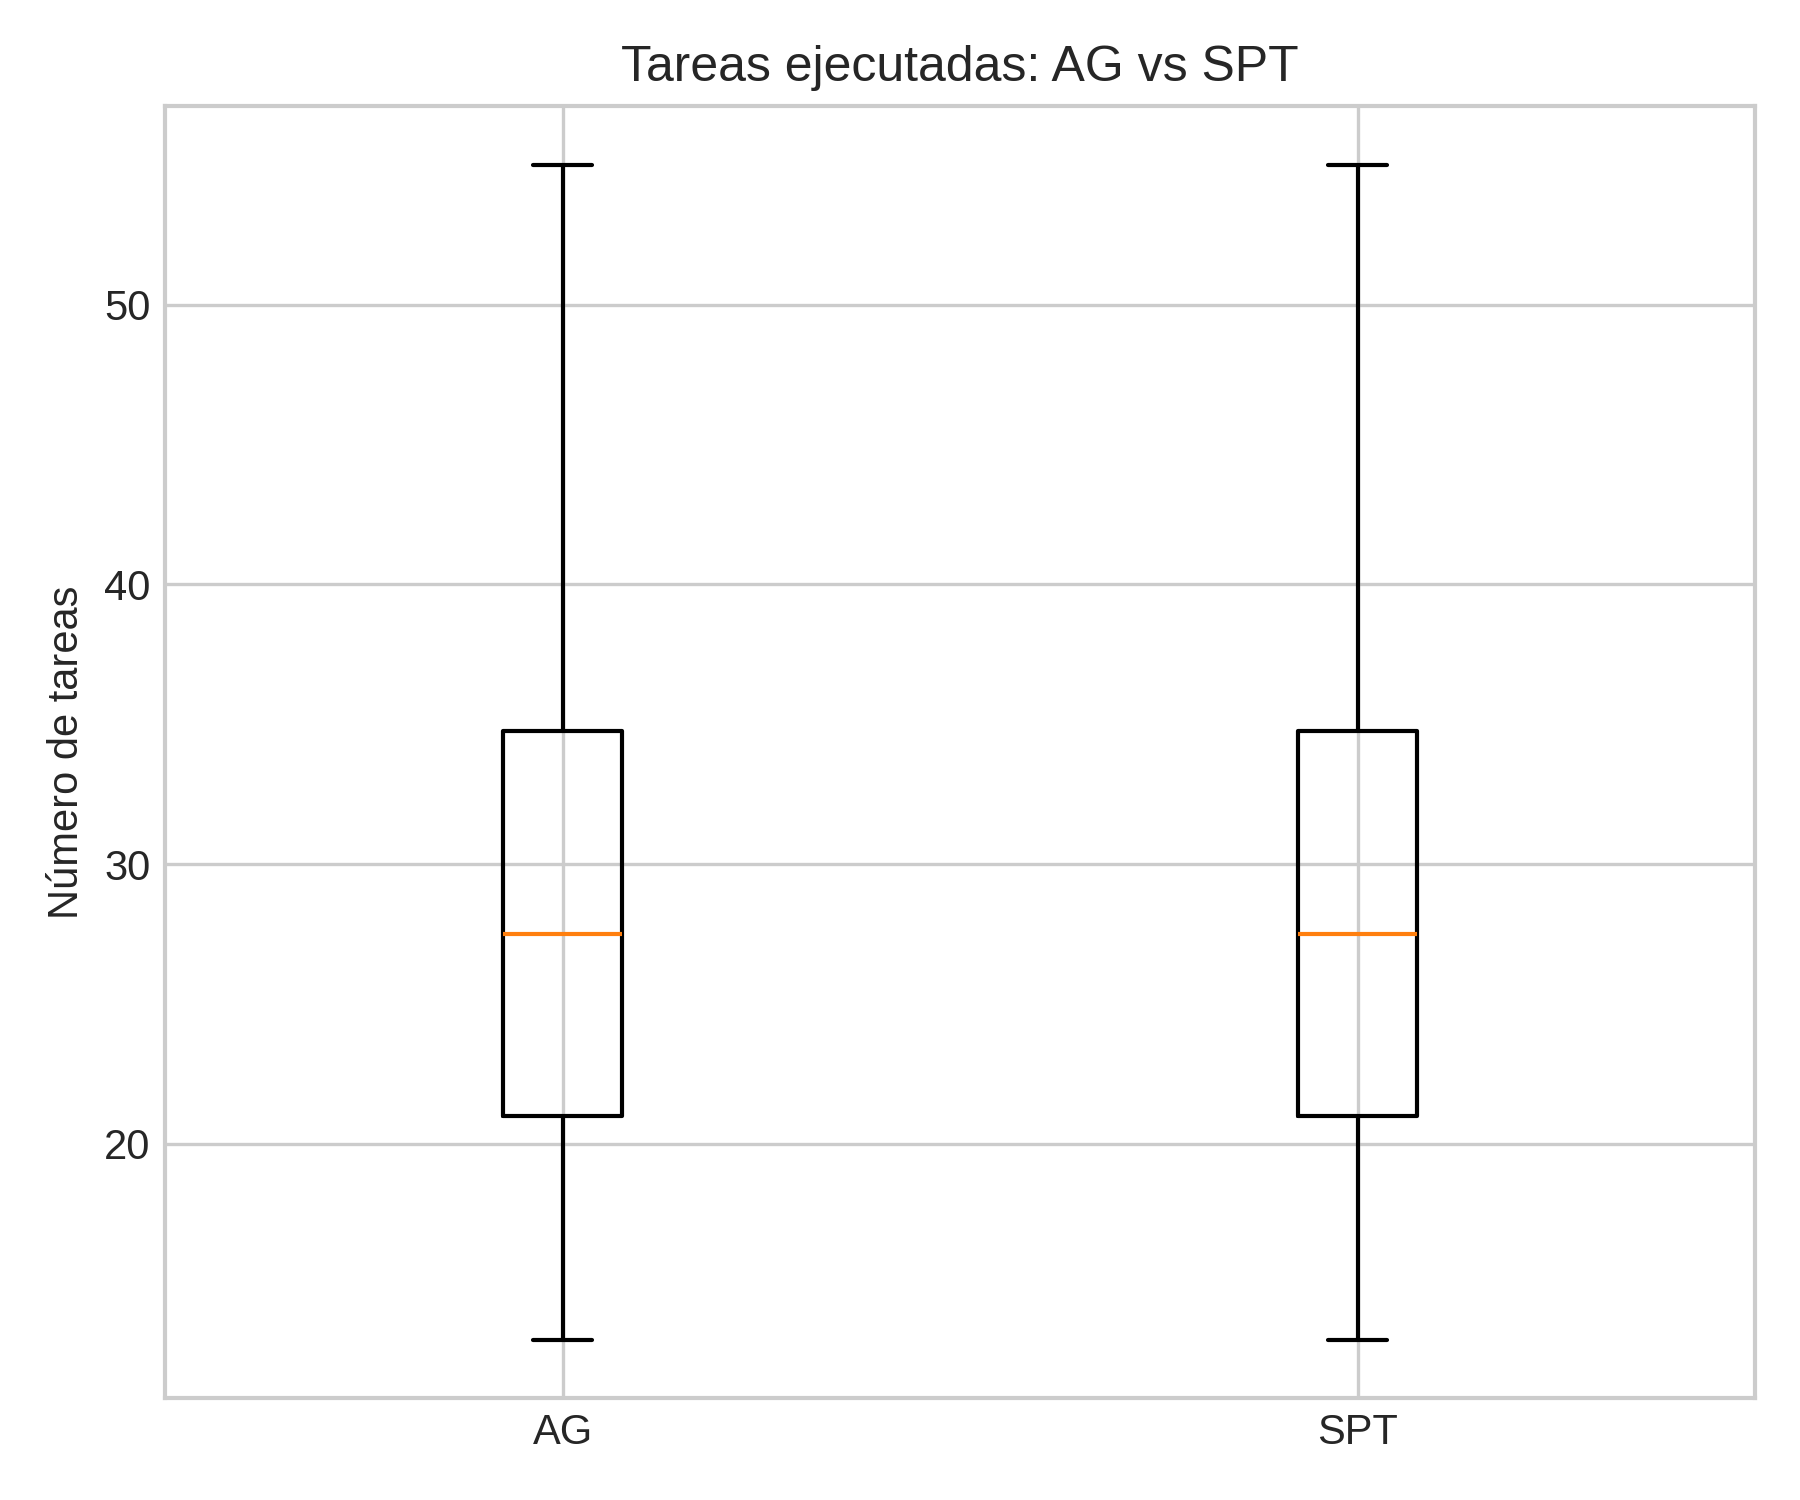
\includegraphics[width=\linewidth]{figures/tareas_ejecutadas.png}
    \caption{Tareas ejecutadas}
\end{subfigure}
\begin{subfigure}{0.45\textwidth}
    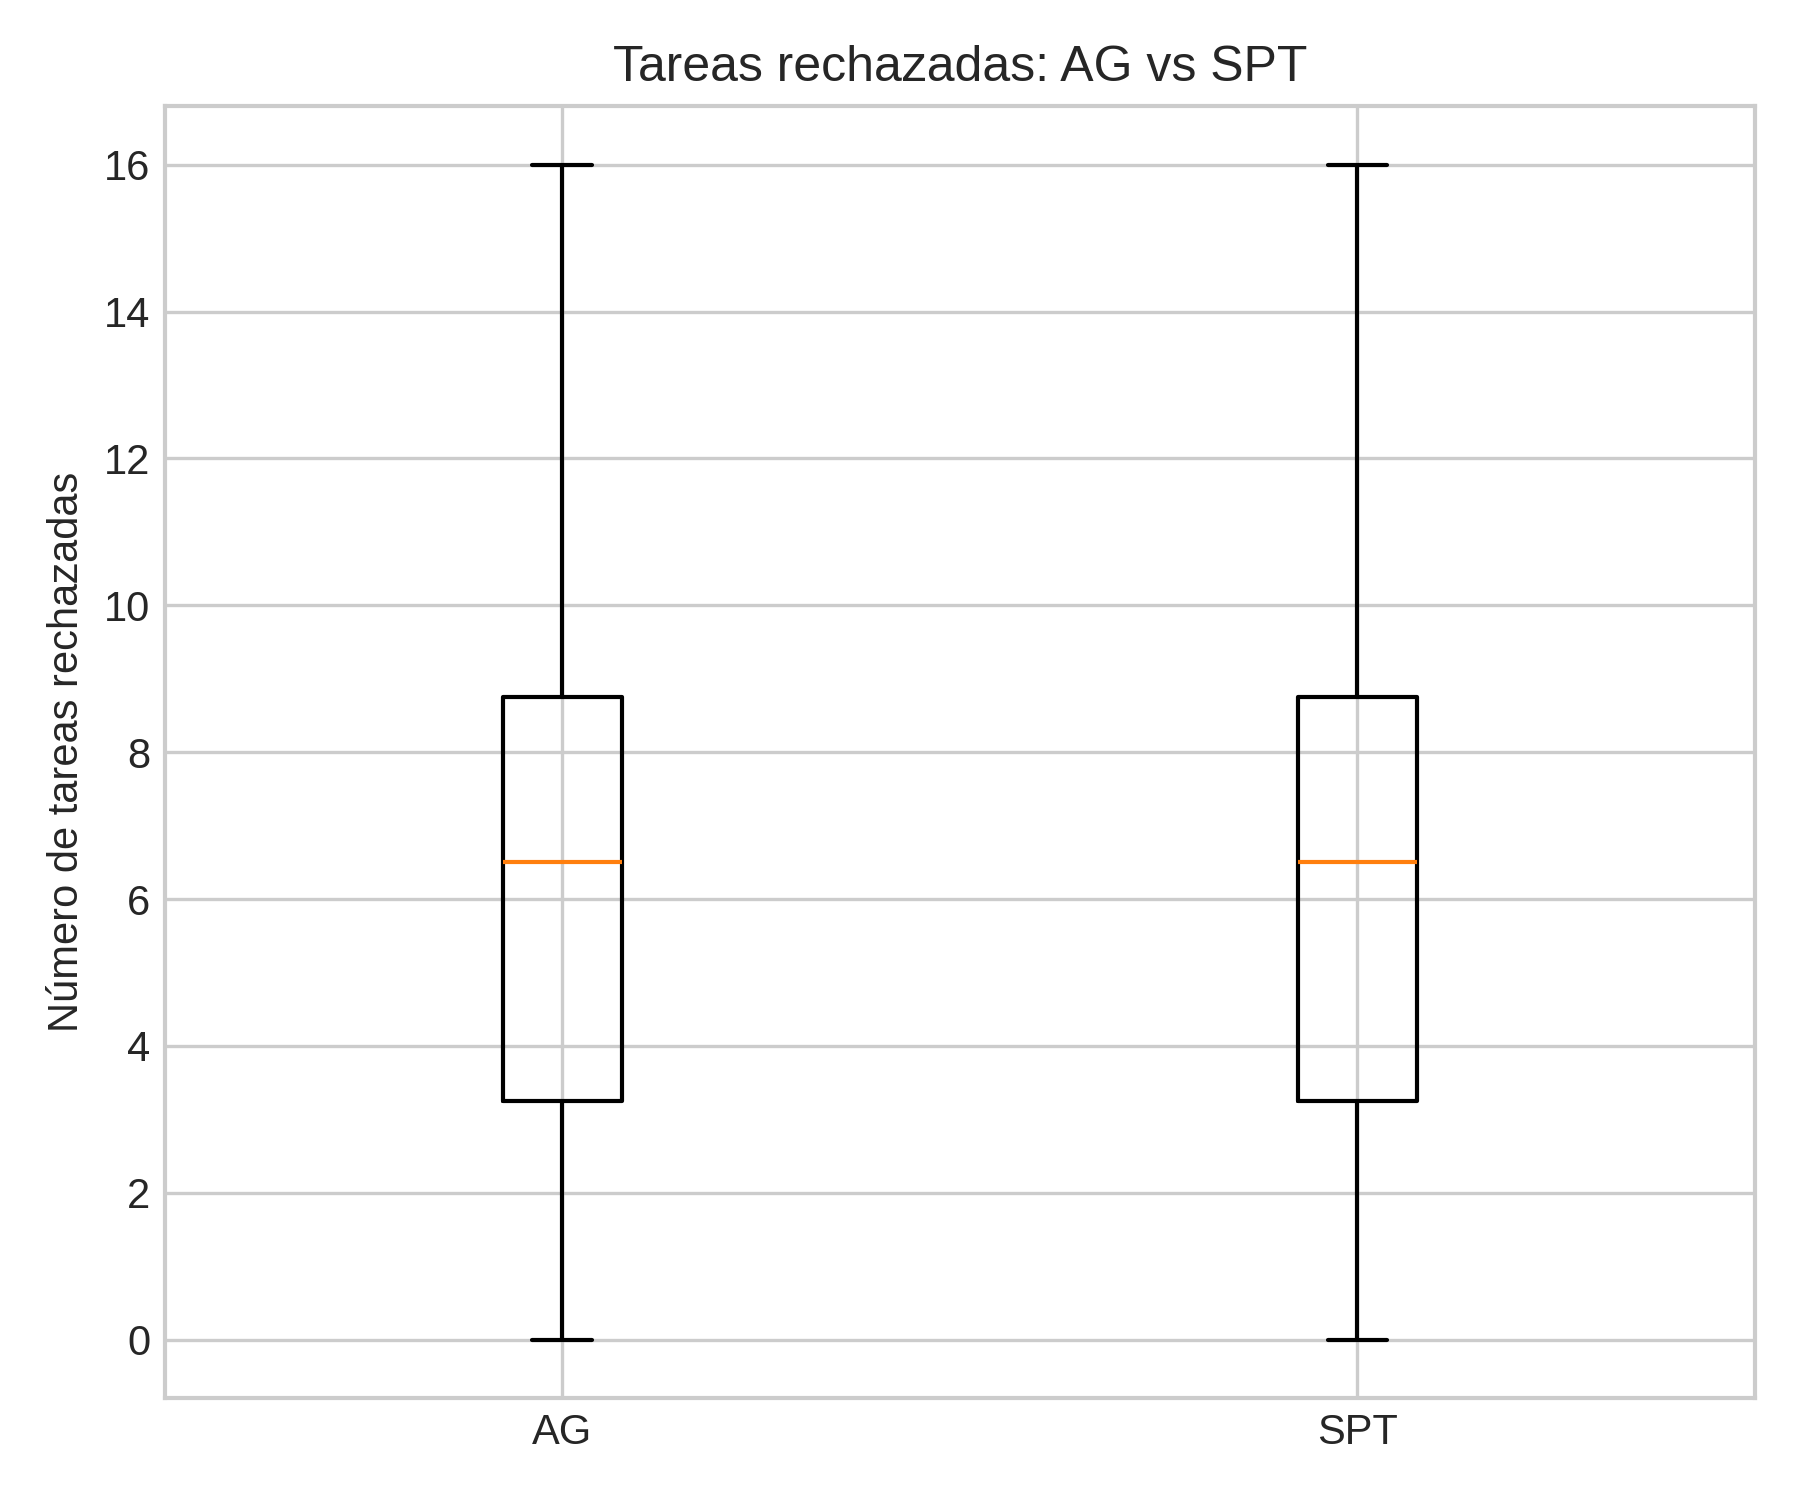
\includegraphics[width=\linewidth]{figures/tareas_rechazadas.png}
    \caption{Tareas rechazadas}
\end{subfigure}
\caption{Distribución comparativa de tareas ejecutadas y rechazadas.}
\label{fig:tareas-ejecutadas-rechazadas}
\end{figure}

Las distribuciones confirman que no existe una diferencia sistemática entre AG y SPT en cuanto al número de tareas completadas. Ambas técnicas logran niveles similares de factibilidad bajo las mismas restricciones del simulador.

% -------------------------------------------------------------------
\subsection{Tareas ejecutadas y rechazadas}
Aunque los promedios son iguales, la variabilidad es distinta: el AG presenta colas más compactas en sus distribuciones, lo que indica mayor estabilidad entre instancias. Desde la perspectiva del taller, esto significa cronogramas más predecibles y menor sensibilidad a la estructura de cada día de trabajo.

Las tareas rechazadas también muestran comportamientos equivalentes en promedio, aunque con ligera tendencia de SPT a rechazar más tareas en instancias con muchas precedencias o restricciones de repuestos, dado que su ordenamiento exclusivamente basado en tiempos no siempre respeta la secuencia lógica más adecuada.

% -------------------------------------------------------------------
\subsection{Sobrecarga vs eficiencia del sistema}

\begin{figure}[H]
\centering
\begin{subfigure}{0.45\textwidth}
    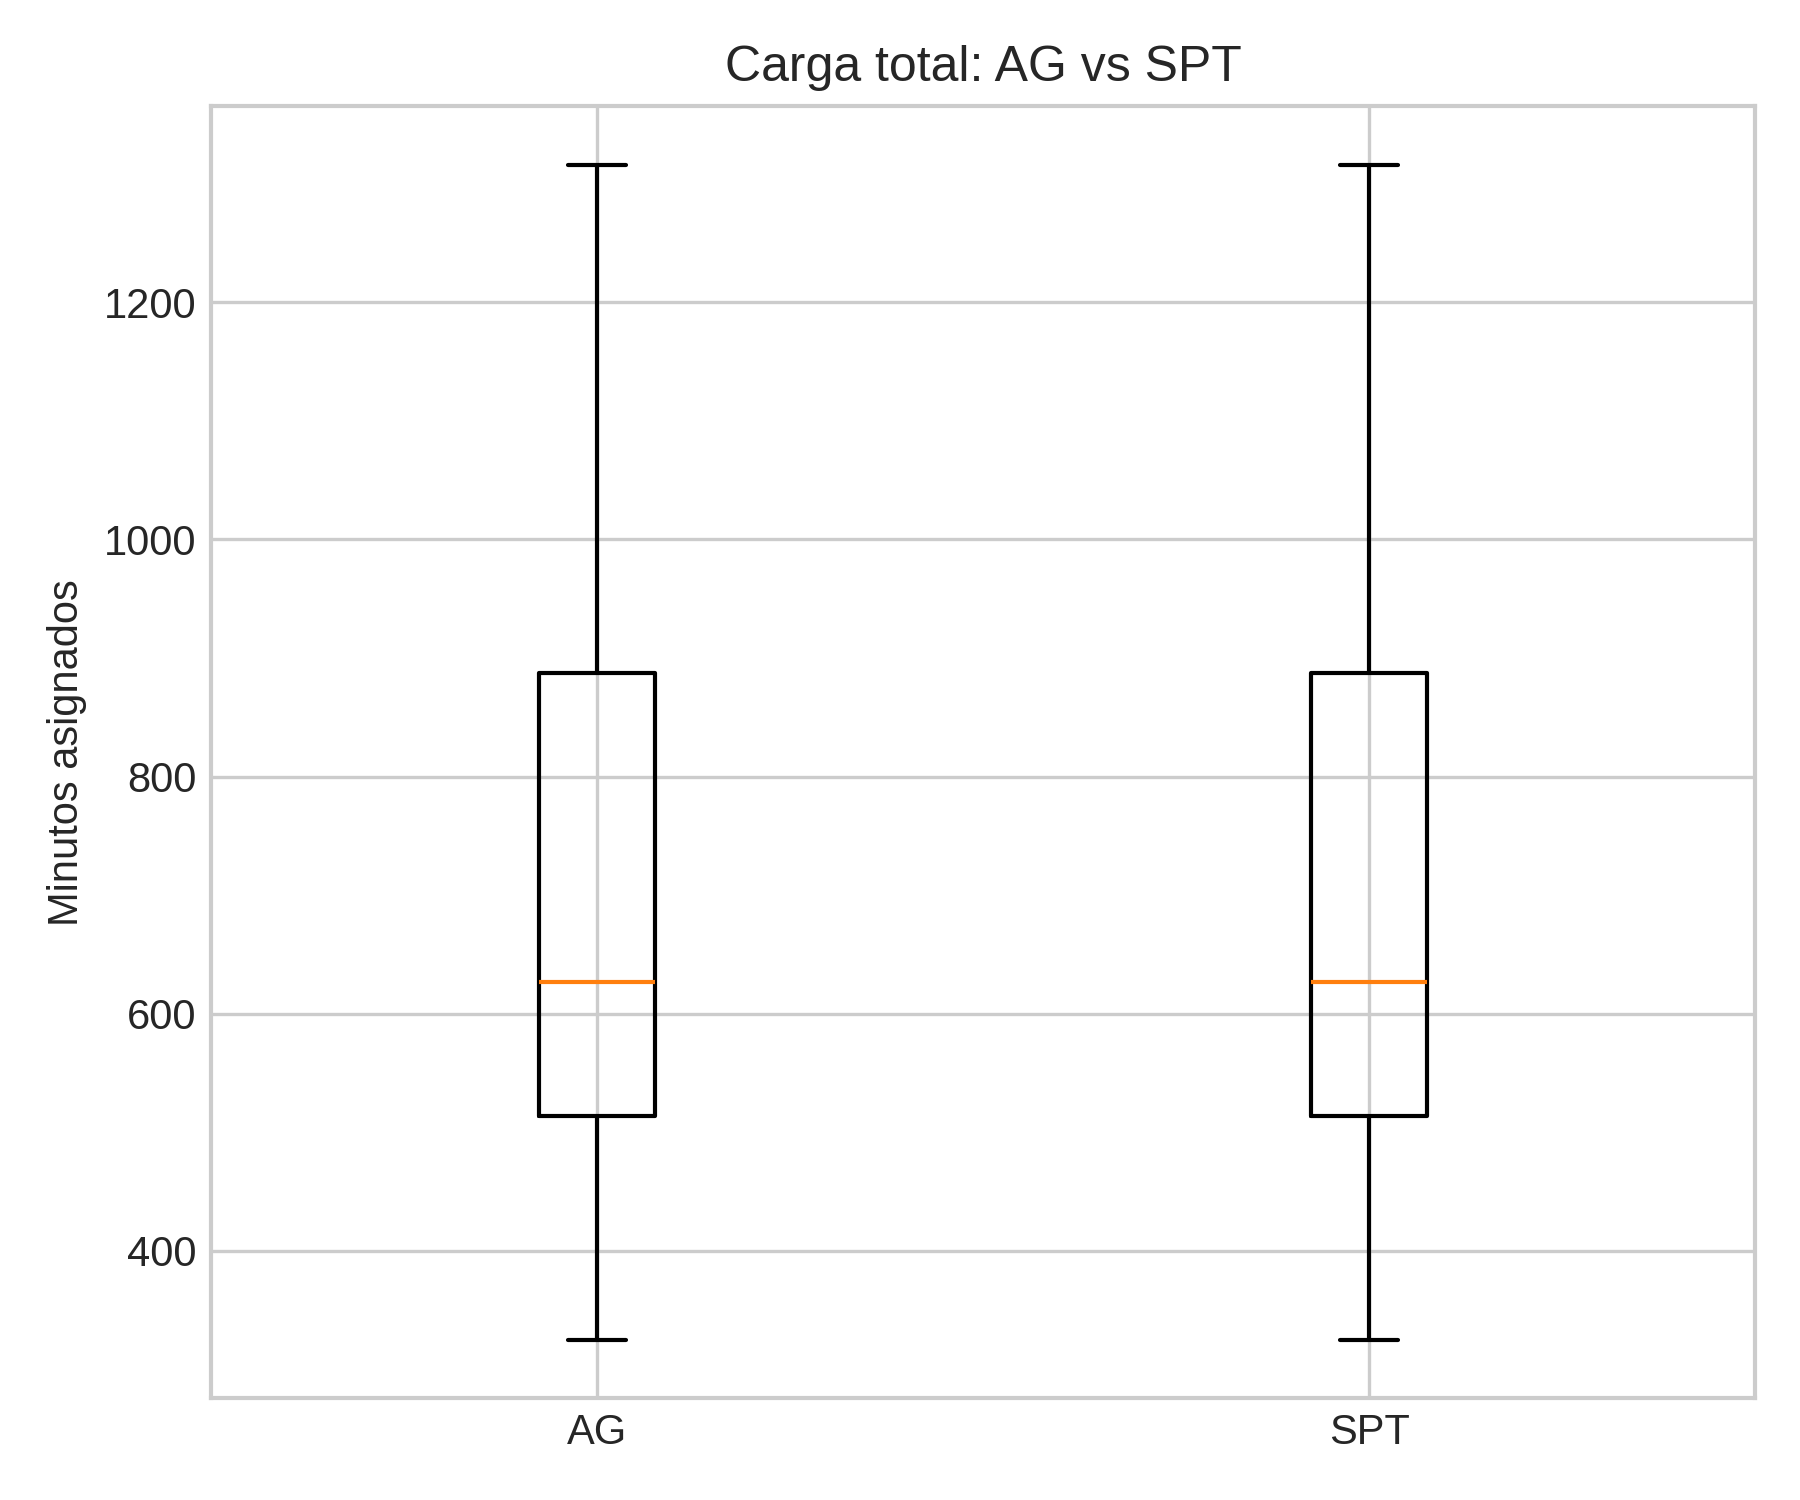
\includegraphics[width=\linewidth]{figures/carga_total.png}
    \caption{Carga total}
\end{subfigure}
\begin{subfigure}{0.45\textwidth}
    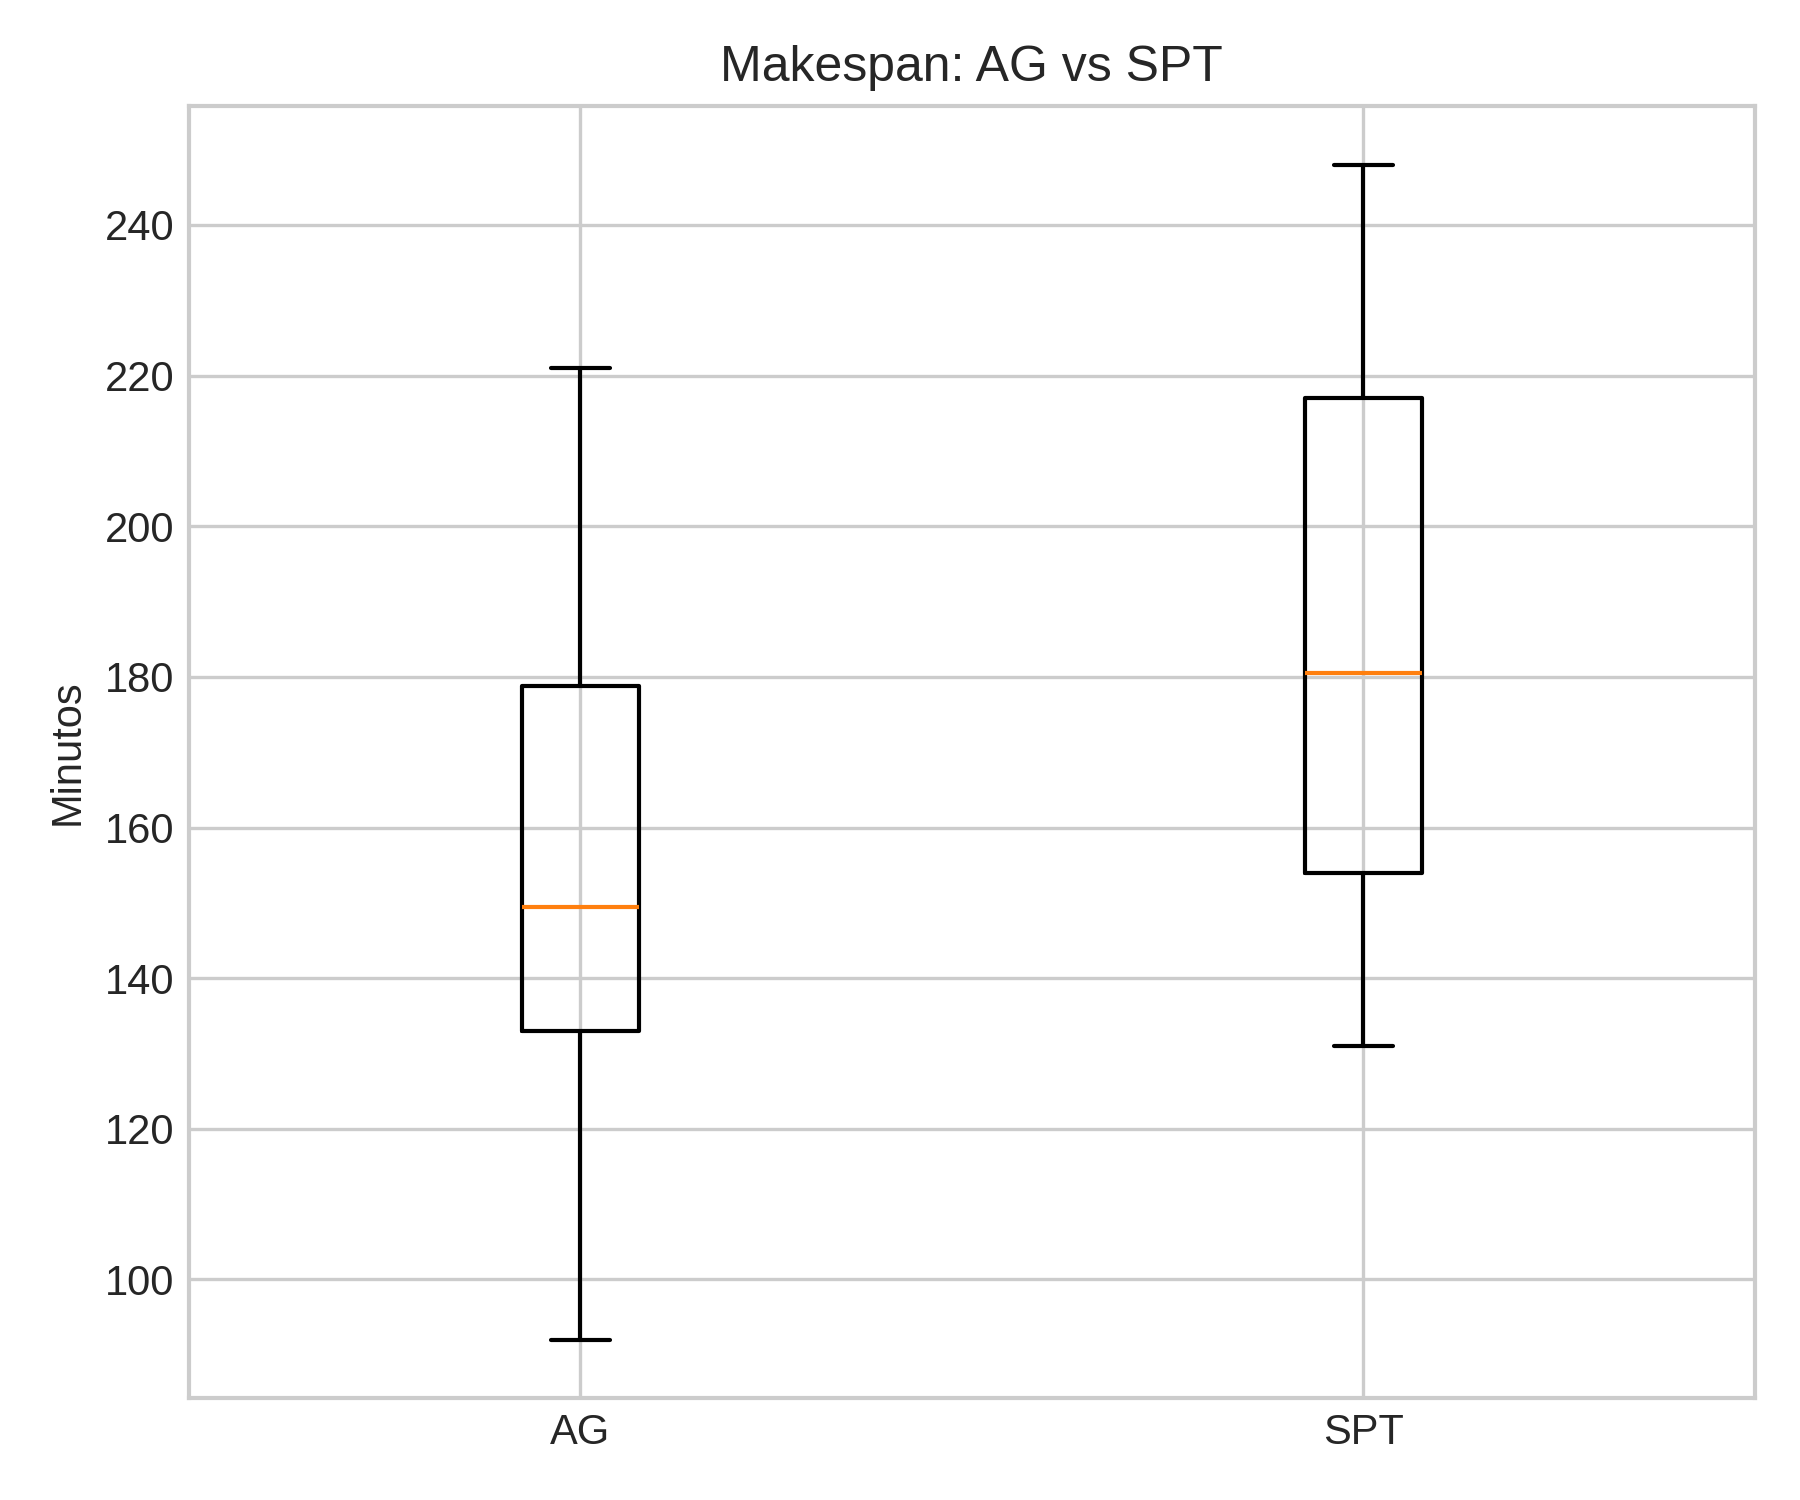
\includegraphics[width=\linewidth]{figures/makespan.png}
    \caption{Makespan}
\end{subfigure}
\caption{Uso del horizonte temporal y eficiencia global.}
\label{fig:carga-makespan}
\end{figure}

Aunque la carga total es idéntica entre algoritmos (resultado que depende directamente del número de tareas ejecutadas), el makespan del AG es mucho menor. Esto implica que el AG logra acomodar la misma cantidad de trabajo en un tiempo efectivo significativamente más corto. Industrialmente, esto se traduce en:

\begin{itemize}
    \item menor tiempo muerto entre tareas,
    \item mejores secuencias internas,
    \item menor fragmentación del trabajo,
    \item cronogramas con menos huecos entre operaciones.
\end{itemize}

El SPT, al priorizar únicamente tareas cortas, puede inducir solapamientos ineficientes o asignaciones subóptimas que extienden el makespan total.

% -------------------------------------------------------------------
\subsection{Balance entre operarios}

\begin{figure}[H]
\centering
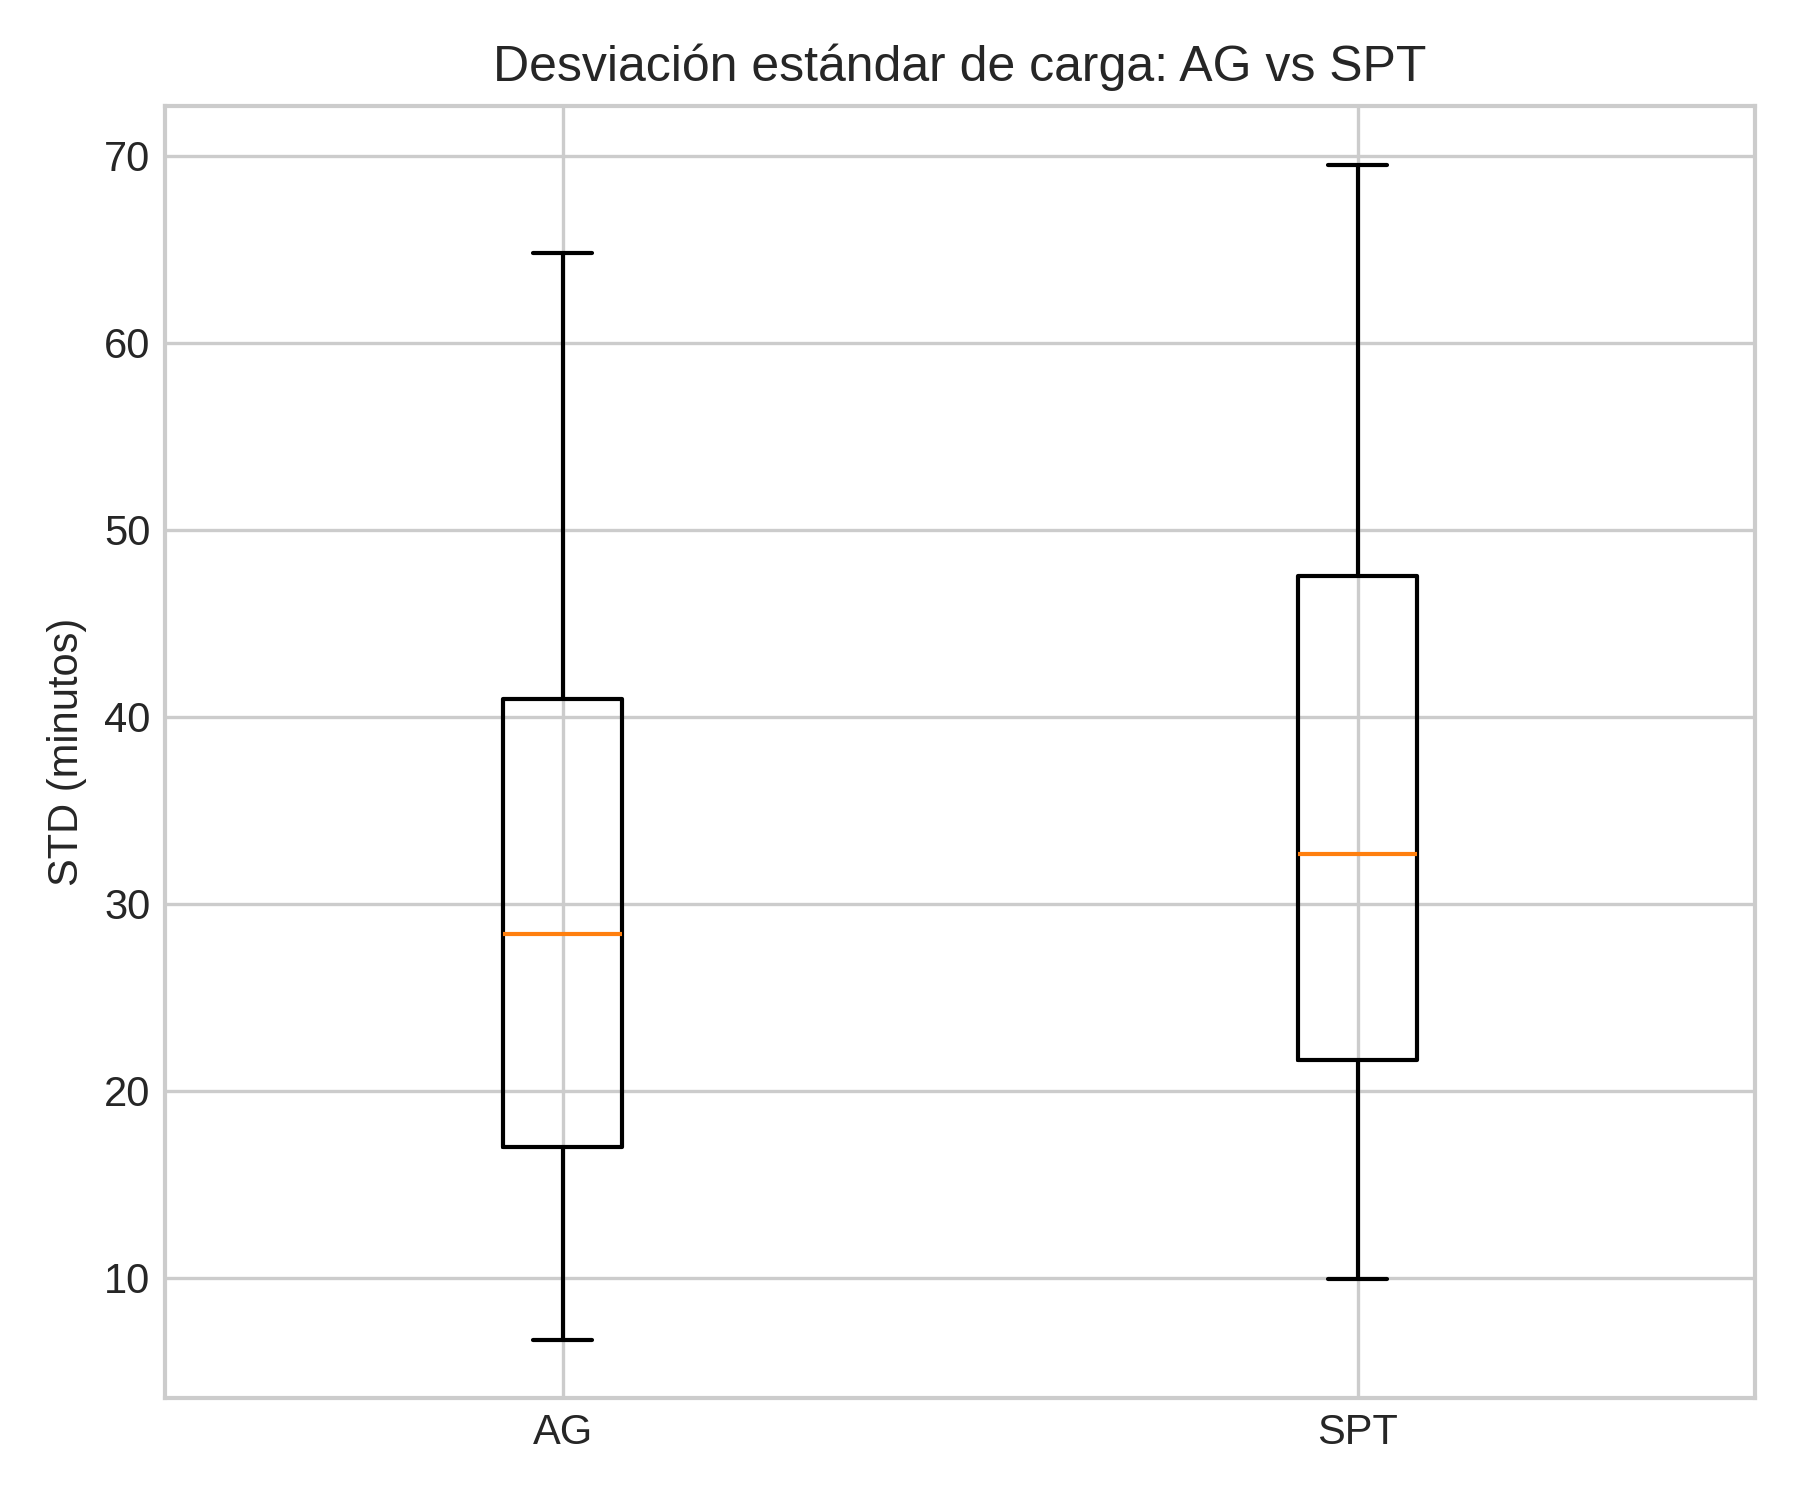
\includegraphics[width=0.55\textwidth]{figures/carga_std.png}
\caption{Desviación estándar de carga entre operarios.}
\label{fig:std-carga}
\end{figure}

El AG obtiene una desviación estándar notablemente menor, lo que indica un reparto más equilibrado del trabajo. Esta mejora no surge por casualidad, sino porque:

\begin{itemize}
    \item la función de aptitud penaliza explícitamente la mala distribución de carga,
    \item la representación del individuo codifica simultáneamente prioridades y asignación de operarios,
    \item la presión selectiva del AG favorece naturalmente soluciones más balanceadas.
\end{itemize}

Para el taller, un mejor balance significa menor riesgo de cuellos de botella, reducción de sobrecarga individual y mayor estabilidad operativa.

% -------------------------------------------------------------------
\subsection{Análisis del tiempo de ejecución}

Con el fin de cuantificar el costo computacional de ambos enfoques, se ejecutó un experimento
controlado sobre 10 instancias generadas con semilla fija (\textit{seed} = 42), cada una con
2 órdenes de trabajo. La Tabla~\ref{tab:tiempos_ejecucion} resume los estadísticos descriptivos
de los tiempos de ejecución por algoritmo.

\begin{table}[H]
\centering
\caption{Comparación de tiempos de ejecución entre AG y SPT (10 instancias, 2 OT por instancia, \textit{seed} = 42).}
\label{tab:tiempos_ejecucion}
\begin{tabular}{lccccc}
\toprule
Algoritmo & Promedio (s) & Mediana (s) & Mínimo (s) & Máximo (s) & Desv. Est. (s) \\
\midrule
AG  & 3.1284 & 2.9697 & 2.6971 & 3.7797 & 0.3907 \\
SPT & 0.000103 & 0.000103 & 0.000088 & 0.000124 & 0.0000099 \\
\bottomrule
\end{tabular}
\end{table}

Los resultados muestran que SPT presenta tiempos prácticamente instantáneos (del orden de
\(10^{-4}\) segundos), comportamiento coherente con una heurística determinística de baja complejidad.
En contraste, el AG requiere en promedio 3.13 segundos por instancia, debido a la evaluación
iterativa de poblaciones durante el proceso evolutivo (300 generaciones y 100 individuos por
población en la configuración final). Aunque este costo es mayor que el de SPT, sigue siendo
operativamente bajo para los tamaños de instancia evaluados y compatible con una planeación diaria.

% -------------------------------------------------------------------
\subsection{Ventajas y desventajas de cada enfoque}

\paragraph{Algoritmo Genético (AG):}  
\begin{itemize}
    \item \textbf{Ventajas:}
    \begin{itemize}
        \item Menor makespan.
        \item Mejor balance de carga.
        \item Mayor estabilidad entre instancias.
        \item Capacidad para capturar interacciones complejas entre precedencias, operarios y repuestos.
    \end{itemize}
    \item \textbf{Desventajas:}
    \begin{itemize}
        \item Mayor tiempo de cómputo que SPT.
        \item Requiere calibración de parámetros.
    \end{itemize}
\end{itemize}

\paragraph{SPT:}
\begin{itemize}
    \item \textbf{Ventajas:}
    \begin{itemize}
        \item Simplicidad y rapidez de ejecución.
        \item Funciona razonablemente bien en entornos con pocas restricciones internas.
    \end{itemize}
    \item \textbf{Desventajas:}
    \begin{itemize}
        \item No integra precedencias de manera natural.
        \item Puede generar secuencias ineficientes y un makespan elevado.
        \item Tiende a desequilibrar la carga entre operarios.
    \end{itemize}
\end{itemize}

% -------------------------------------------------------------------
\section{Discusión de los Hallazgos e Implicaciones}

Los experimentos demuestran que, aunque el AG y el SPT ejecutan en promedio la misma cantidad de tareas, el AG produce cronogramas significativamente más eficientes. El makespan menor y la mejor distribución del trabajo son evidencia de que el AG es capaz de capturar estructuras profundas del problema que SPT ignora debido a su simplicidad.

Desde una perspectiva industrial, esto implica:

\begin{itemize}
    \item Mayor capacidad de respuesta del taller.
    \item Horarios más compactos, que permiten atender trabajos urgentes dentro del mismo día.
    \item Menor dependencia del criterio manual o del orden de llegada.
    \item Mejor utilización del equipo humano disponible.
\end{itemize}

En conclusión, el AG no solo es competitivo frente al SPT, sino que lo supera en los aspectos más relevantes para la operación diaria del taller, justificando el uso de técnicas evolutivas en problemas reales de programación de tareas.

\chapter{Conclusiones}

Se alcanzó exitosamente el objetivo general: desarrollar un modelo de automatización basado en algoritmos genéticos para la asignación de tareas en un ERP de talleres industriales, comparándolo con el método SPT bajo condiciones reproducibles.

\textbf{Implementación del Algoritmo Genético.} Se desarrolló un AG con representación dual (asignación de operarios + prioridades de secuenciación), función de aptitud ponderada y operadores genéticos calibrados (300 generaciones, 15\% mutación, selección por ranking). El modelo es escalable, reproducible y ejecutable en tiempos prácticos.

\textbf{Desempeño Comparativo.} Aunque AG y SPT ejecutan idéntico número de tareas (29.53 promedio en 30 instancias), el AG demuestra superior estructuración: makespan 15.6\% menor (157.37 vs 186.53 minutos) y balance de carga 14.3\% mejor (desviación estándar 30.10 vs 35.11). Esta eficiencia genera valor industrial mediante cronogramas más compactos y distribución equitativa de trabajo.

\textbf{Impacto Industrial.} La reducción del 15.6\% en makespan representa 29.16 minutos diarios de eficiencia adicional, equivalente a 117.6 horas anuales (aproximadamente 15 días de productividad sin incremento de recursos). El mejor balance reduce cuellos de botella, fatiga del personal y errores operativos. Para Rectificadora Recti-Ram, esto implica mayor flexibilidad operativa, cumplimiento de plazos más confiable y capacidad para aceptar mayor volumen de órdenes.

\textbf{Validez Técnica.} El modelo formalizado proporciona marco riguroso. La validación experimental confirma: (1) Convergencia rápida en 300 generaciones; (2) Factibilidad de todas las soluciones bajo restricciones reales; (3) Estabilidad superior a SPT; (4) Reproducibilidad completa mediante semilla aleatoria fija y documentación detallada.

\textbf{Contribuciones.} El proyecto formaliza empíricamente un problema de asignación en contexto ERP real, demostrando que técnicas evolutivas superan heurísticas clásicas en este dominio. Proporciona metodología reproducible aplicable a PYMES mediante software de código abierto (Python, PyGAD), reduciendo barreras de adopción.

\textbf{Oportunidades Futuras.} Las limitaciones abren oportunidades de extensión: (1) Modelos híbridos AG-PSO o AG-ACO; (2) Job Shop Scheduling flexible con selección dinámica de máquinas; (3) Optimización multiobjetivo integrando inventarios y costos; (4) Aprendizaje automático para ajuste dinámico de parámetros; (5) Integración con IoT e Industria 4.0; (6) Computación cuántica (quantum annealing) para instancias mayores.

\textbf{Conclusión Final.} Los algoritmos genéticos demuestran ser herramienta viable para automatizar asignación de tareas industriales. Su superior desempeño respecto a SPT, adaptabilidad y reproducibilidad los posicionan como componente valiosa en sistemas de soporte de decisión operacional. Sin embargo, la implementación exitosa requiere comprensión profunda del dominio, validación rigurosa en ambiente real, diálogo continuo con usuarios finales y compromiso con mejora iterativa. La evolución natural del trabajo conduce hacia técnicas híbridas, modelos flexibles de Job Shop, integración con ERP e IoT, y arquitecturas emergentes como aprendizaje automático y computación cuántica, posicionando este aporte en la frontera de tecnologías emergentes en optimización industrial.

\chapter{Trabajo Futuro}

\section{Optimización del algoritmo genético}
\section{Sistemas híbridos}
\section{Integración con el ERP}
\section{Pruebas con datos reales históricos}
\chapter{Glosario}

Este glosario presenta términos especializados y conceptos clave que requieren aclaración rápida, complementando las explicaciones detalladas proporcionadas en capítulos anteriores. Se omiten intencionalmente conceptos que ya han sido formalmente definidos o desarrollados extensamente.

\section*{Conceptos Fundamentales de Optimización}

\begin{description}
    \item[Optimización:] Proceso de encontrar la mejor solución posible (o cercana a ella) entre un conjunto de alternativas, generalmente minimizando o maximizando una función objetivo sujeta a restricciones.
    
    \item[Heurística:] Técnica de resolución de problemas que utiliza reglas prácticas o intuición para encontrar soluciones buenas rápidamente, sin garantizar que sean óptimas pero con menor costo computacional que métodos exactos.
    
    \item[Metaheurística:] Estrategia general de búsqueda de alto nivel que guía el proceso de exploración del espacio de soluciones, permitiendo combinar diferentes técnicas de optimización para escapar de óptimos locales.
    
    \item[Óptimo local:] Solución mejor que todas sus alternativas inmediatas en el espacio de búsqueda, pero no necesariamente la mejor solución global.
    
    \item[Óptimo global:] Mejor solución posible en todo el espacio de búsqueda.
    
    \item[NP-hard:] Clase de problemas computacionales cuya dificultad es tal que no se conoce algoritmo polinomial para resolverlos, haciendo que heurísticas y metaheurísticas sean alternativas viables.
\end{description}

\section*{Problemas de Programación Clásicos}

\begin{description}
    \item[Flow Shop:] Problema de programación donde múltiples trabajos deben pasar por una secuencia fija de máquinas en el mismo orden.
    
    \item[Job Shop:] Problema de programación donde múltiples trabajos tienen rutas específicas pero potencialmente diferentes a través de un conjunto de máquinas.
    
    \item[Flexible Job Shop:] Variante del Job Shop donde cada operación puede ser realizada por una de varias máquinas alternativas.
    
    \item[Shortest Processing Time (SPT):] Regla de despacho que prioriza tareas con menor tiempo de procesamiento, comúnmente usada como punto de referencia en ingeniería industrial. Fue adoptada en este trabajo como método de comparación contra el algoritmo genético.
    
    \item[Task Assignment Problem (TAP):] Problema de optimización que consiste en asignar un conjunto de tareas a un conjunto de operarios o recursos disponibles. Este trabajo es una variante específica del TAP con restricciones industriales.
    
    \item[Greedy:] Estrategia algorítmica que toma decisiones localmente óptimas en cada paso sin considerar el impacto global, típica de métodos como SPT.
\end{description}

\section*{Conceptos de Ingeniería Industrial y Sistemas ERP}

\begin{description}
    \item[Automatización:] Uso de sistemas técnicos o computacionales para ejecutar procesos sin intervención manual directa, mejorando eficiencia y consistencia.
    
    \item[ERP (Enterprise Resource Planning):] Sistema integrado de gestión empresarial que centraliza información de procesos operativos, financieros y administrativos. En este contexto, nos enfocamos en el módulo de asignación de tareas.
    
    \item[Sistema de soporte de decisión:] Herramienta computacional diseñada para asistir a gerentes y operarios en la toma de decisiones complejas proporcionando análisis y recomendaciones.
    
    \item[Cuello de botella (Bottleneck):] Recurso o tarea que limita la capacidad de producción debido a su disponibilidad limitada o tiempo de procesamiento excesivo.
    
    \item[Eficiencia operativa:] Medida de qué tan bien se utilizan los recursos disponibles para lograr los objetivos de producción.
    
    \item[Productividad:] Cantidad de salida (tareas completadas, productos generados) por unidad de entrada (tiempo, recursos).
    
    \item[ROI (Return on Investment):] Indicador financiero que mide el retorno generado por una inversión en relación con su costo. En este estudio se estimó una recuperación entre 6-12 meses.
\end{description}

\section*{Términos Técnicos Complementarios}

\begin{description}
    \item[PyGAD:] Biblioteca de código abierto en Python que proporciona implementaciones de algoritmos genéticos. Utilizada en este trabajo para la implementación del AG.
    
    \item[Calibración empírica:] Ajuste de parámetros basado en experimentación práctica para encontrar valores que produzcan buen desempeño. En este proyecto se realizó en el Capítulo 6.
    
    \item[Instancia de problema:] Conjunto específico de datos (tareas, operarios, restricciones) que define una situación particular del problema a resolver. Se utilizaron 30 instancias independientes en las pruebas.
    
    \item[Reproducibilidad:] Capacidad de obtener exactamente los mismos resultados en nuevas ejecuciones con los mismos parámetros e información de control. Este proyecto garantiza reproducibilidad mediante semilla aleatoria fija (seed=42).
    
    \item[Escalabilidad:] Capacidad de una técnica o algoritmo para mantener su eficiencia al resolver instancias de mayor tamaño. El AG propuesto escala polinomialmente con el número de tareas.
    
    \item[Robustez:] Capacidad de un algoritmo para producir soluciones de calidad consistente bajo variaciones en parámetros o datos de entrada.
    
    \item[Estabilidad:] Propiedad de producir resultados similares en múltiples ejecuciones independientes con los mismos parámetros. El AG mostró desviación estándar del 14.3\% en los resultados.
    
    \item[Convergencia rápida:] Capacidad del algoritmo de alcanzar soluciones de alta calidad en pocas generaciones. El AG converge en 300 generaciones (aproximadamente 2 minutos por ejecución).
\end{description}

\section*{Conceptos Estadísticos y de Análisis}

\begin{description}
    
    \item[Mejora relativa:] Porcentaje de cambio en una métrica al comparar dos métodos. El AG logró 15.6\% de mejora en makespan respecto a SPT.
    
    \item[Tiempo de ejecución:] Cantidad de tiempo de procesamiento requerida por un algoritmo para resolver una instancia del problema.
    
    \item[Complejidad computacional:] Estimación del uso de recursos (tiempo y memoria) que requiere un algoritmo en función del tamaño de la entrada.
    
    \item[Desviación estándar:] Medida estadística de variabilidad en un conjunto de datos. En este trabajo se utilizó para cuantificar el balance de carga entre operarios.
\end{description}

\section*{Abreviaciones Técnicas Frecuentes}

\begin{description}
    \item[AG:] Algoritmo Genético.
    
    \item[SPT:] Shortest Processing Time.
    
    \item[TAP:] Task Assignment Problem.
    
    \item[OT:] Orden de Trabajo.
    
    \item[ERP:] Enterprise Resource Planning (Sistema de Planificación de Recursos Empresariales).
    
    \item[PyGAD:] Python Genetic Algorithm for Database.
\end{description}

% --------- Bibliografía ---------
\cleardoublepage
\printbibliography

% --------- Anexos ---------
\appendix
\include{anexos/A-datos}
\include{anexos/B-codigo}

\end{document}